%==============================================================
% CO3 Project Report  --  MSLS 2026
% Fair Water Distribution in Rural Nepal:
% Lagrange-Newton vs. Simulated Annealing
%
% Single-column, T1-style ZHAW title page,
% max. 4 pages of body content (intro - conclusion),
% code listing + references in the appendix.
%==============================================================
\documentclass[
    11pt,
    english,
    singlespacing,
    parskip,
    headsepline,
    consistentlayout,
    oneside,
]{MastersDoctoralThesis}

\usepackage{float}
\usepackage{caption}
\captionsetup{
  justification=justified,
  singlelinecheck=false,
  format=hang,
  font=small,
  labelfont=bf
}

%----------------------------------------------------------------------------------------
% PREAMBLE: PACKAGES AND CONFIGURATIONS
%----------------------------------------------------------------------------------------

\usepackage[utf8]{inputenc}
\usepackage[T1]{fontenc}
\usepackage{amsmath,amsfonts,amssymb,amscd,amsthm,xspace}
\usepackage{graphicx}
\usepackage{booktabs}
\usepackage{algorithm}
\usepackage{algpseudocode}
% \usepackage{cite}     % replaced by natbib in main.tex
\usepackage{csquotes}

% Hyperlinks
\usepackage{hyperref}
\hypersetup{
    colorlinks=true,
    linkcolor=blue,
    citecolor=blue,
    urlcolor=blue,
}

\usepackage{caption}
\captionsetup{format=hang,font=small}
\usepackage{setspace}
\usepackage{siunitx}
\usepackage{multirow}
\usepackage{longtable}
\usepackage{pdfpages}
\usepackage[toc,page]{appendix}


% --- citations: IEEE numeric style ---------------------------------
\usepackage[numbers,sort&compress]{natbib}

% --- code listings -----------------------------------------------------------
\usepackage{listings}
\usepackage{xcolor}
\definecolor{codegray}{rgb}{0.95,0.95,0.95}
\definecolor{codekeyword}{rgb}{0.00,0.35,0.70}
\definecolor{codestring}{rgb}{0.55,0.20,0.20}
\definecolor{codecomment}{rgb}{0.35,0.55,0.35}
\lstdefinestyle{pythonstyle}{
    language=Python,
    backgroundcolor=\color{codegray},
    basicstyle=\ttfamily\footnotesize,
    keywordstyle=\color{codekeyword}\bfseries,
    stringstyle=\color{codestring},
    commentstyle=\color{codecomment}\itshape,
    numbers=left,
    numberstyle=\tiny\color{gray},
    stepnumber=1,
    numbersep=8pt,
    breaklines=true,
    breakatwhitespace=true,
    showstringspaces=false,
    frame=single,
    framerule=0.3pt,
    rulecolor=\color{gray!40},
    xleftmargin=12pt,
    xrightmargin=4pt,
    tabsize=4,
    captionpos=b,
}
\lstset{style=pythonstyle}

% --- project metadata --------------------------------------------------------
\thesistitle{Fair Water Distribution in Rural Nepal: A~Comparison of Lagrange--Newton and Simulated Annealing}
\author{Triantafyllia Giora, Spyridon Margomenos, Nicolas Biner, Robin Giacomelli}
\university{Zurich University of Applied Sciences}
\department{School of Life Sciences and Facility Management}
\subject{Applied Computational Life Sciences}

\AtBeginDocument{
  \hypersetup{pdftitle={CO3 Project -- Fair Water Distribution in Rural Nepal}}
  \hypersetup{pdfauthor={Giora, Margomenos, Biner, Giacomelli}}
}

\newcommand{\TODO}[1]{\textcolor{red}{[TODO: #1]}}

\begin{document}

\pagestyle{plain}

%==============================================================
% TITLE PAGE  (T1-style ZHAW layout, adapted from Front/titlepage.tex)
%==============================================================
\newgeometry{margin=1in}
\begin{titlepage}
\setlength{\parskip}{0pt}

\begin{center}

\includegraphics[width=0.15\textwidth]{Figures/zhaw_rgb}

\ifxetex
    \vspace{0.5cm}
    {\zhawtitlefont\color{zhawblue}\LARGE \univname\par}
    \vspace{0.2cm}
\else
    \vspace{0.75cm}
    {
\includegraphics[height=17.9pt]{Figures/zhaw_font_eng_font}\par}
    \vspace{0.05cm}
\fi
{\Large Department \deptname\par}
\vspace{0.15cm}
{\Large Institute of Computational Life Sciences\par}
\vspace{2.5cm}
\textsc{\Large CO3 Project Report -- Spring Semester 2026}
\vspace{0.2cm}
\HRule\\[0.4cm]
{\Large\bfseries Fair Water Distribution in Rural Nepal:\\[2pt]
A Comparison of Lagrange--Newton and Simulated Annealing\par}
\vspace{0.4cm}
\HRule\\[1.2cm]

\begin{center}
    \large
    \emph{Authors:}\\[0.2cm]
    Triantafyllia Giora \\
    Spyridon Margomenos \\
    Nicolas Biner \\
    Robin Giacomelli \\[0.5cm]
    \emph{Lecturer:} \\
    Prof.~Dr.~Thomas Ott \\[0.3cm]
    \emph{Module:} \\
    CO3 -- Optimisation and \\
    Bio-Inspired Algorithms
\end{center}

\vfill

{\large
Submitted on \today\\[0.3cm]
Study program: MSc Applied Computational Life Sciences\\
}

\end{center}
\end{titlepage}
\restoregeometry

%==============================================================
% MAIN MATTER  --  the 4-page report body
%==============================================================
\pagestyle{thesis}
\setcounter{page}{1}

% tighten the body layout: smaller margins & compact chapter heading
\newgeometry{left=2.2cm,right=2.2cm,top=2.2cm,bottom=2.5cm}
% override the class's generous chapter spacing
\renewcommand{\abovechapterskip}{\vspace*{-6pt}}
\renewcommand{\chapterbelowskip}{\vspace*{8pt}}
\renewcommand{\chapterinbetweenskip}{\vspace*{2pt}}
\renewcommand{\chapterfont}{\Large\bfseries}
\renewcommand{\chapterprefixfont}{\normalsize\bfseries}
% reduce paragraph-skip which is generous in the class
\setlength{\parskip}{2pt plus 1pt minus 1pt}

%==============================================================
%  Chapter 1 :  Report body  (Introduction -- Conclusion)
%  Target: four pages in the MastersDoctoralThesis layout.
%==============================================================
\chapter{Fair Water Distribution in Rural Nepal}
\label{chap:report}

%--------------------------------------------------------------
\section{Introduction}
%--------------------------------------------------------------
Access to safe drinking water in rural Nepal remains persistently
constrained by seasonal spring depletion, ageing gravity-fed
infrastructure, and unequal access between households.
Gautam and Dahal~\cite{gautam2020} document that roughly half of Nepal's
community water schemes are non-functional or under-performing,
with weak cost recovery, climate-driven source depletion, and
institutional fragmentation as recurring obstacles. On the
technical side, Laporte et al.~\cite{laporte2022} formulate the post-2015
earthquake restoration of Nepalese gravity-fed networks as a
hierarchical location-allocation and Steiner-forest problem,
solved with a two-phase matheuristic. Both works frame
\emph{infrastructure} and \emph{coverage}; the complementary
operational question of \emph{how to allocate a limited communal
supply once the network is in place} has received less formal
attention.

In this project we take a single village-scale view: given a
fixed daily spring yield and a fixed set of households, how
should the source be split day-by-day? We formulate this as a
small-scale convex quadratic programme with equity weights and
pipe-loss coupling, and we compare two methods from different
classes of the CO3 taxonomy~\citep{ottCO3slides}: a gradient-based
\emph{Lagrange--Newton} solver (Chapters~3--4 of the module) and
the stochastic \emph{Simulated Annealing} metaheuristic
(Chapter~7). The problem is self-formulated, parameterised from
Nepal-specific sources~\citep{nepalDWSS,whoJMP}, and serves as a
compact benchmark on which the two methods can be compared on
accuracy, efficiency and robustness.

%--------------------------------------------------------------
\section{Problem Formulation}
\label{sec:formulation}
%--------------------------------------------------------------

\paragraph{Variables and data.}
Let $x_i$ denote the daily water volume delivered to household
$i \in \{1,\dots,n\}$, $d_i$ its demand, $b_i$ the WHO-aligned
minimum allocation, $a_i \geq 1$ a household-specific
delivery-loss factor (so $a_i x_i$ is the source-side draw
required to deliver $x_i$ at the tap), and $w_i > 0$ a
vulnerability weight that raises the penalty for shortages at
prioritised households. $S$ is the total daily spring yield.
Values (Table~\ref{tab:params}) follow Nepal's Rural Water
Supply Design Standards~\citep{nepalDWSS} and the WHO/JMP
guidelines~\citep{whoJMP}.

\begin{table}[H]
\centering
\small
\caption{Parameters of the base scenario.}
\label{tab:params}
\begin{tabular}{@{}lll@{}}
\toprule
Parameter & Value / range & Source \\ \midrule
Households $n$         & $20$                 & typical rural system size \\
Demand $d_i$           & $225$ \si{L/day}     & SUS $45$ LPCD $\times\, 5$ persons~\citep{nepalDWSS} \\
Minimum $b_i$          & $100$ \si{L/day}     & WHO $20$ LPCD $\times\, 5$ persons~\citep{whoJMP} \\
Loss factor $a_i$      & $[1.00,\, 1.25]$     & pipe / terrain overhead \\
Vulnerability $w_i$    & $[1.00,\, 1.80]$     & equity prioritisation \\
Total supply $S$       & $3500$ \si{L/day}    & scarcity scenario~\citep{gautam2020} \\
\bottomrule
\end{tabular}
\end{table}

\paragraph{Objective.}
We minimise the weighted sum of squared deviations from demand,
\begin{equation}
  f(\mathbf{x}) \;=\; \sum_{i=1}^{n} w_i\bigl(d_i - x_i\bigr)^{2}.
  \label{eq:obj}
\end{equation}
The quadratic form penalises large under-deliveries
super-linearly, and the weights $w_i$ pull the allocation towards
vulnerable households --- an equity mechanism absent from a
uniformly weighted $L_1$ objective $\sum|d_i - x_i|$.
Compared to a Rawlsian max--min criterion~\citep{rawls1971},
the weighted $L_2$ form is smooth and strictly convex,
enabling gradient-based solvers and a unique closed-form
solution~\eqref{eq:waterfilling}; the Rawlsian alternative
is left as a non-smooth extension for future work.

\paragraph{Constraints.}
Mass balance at the source (equality) and box bounds per
household:
\begin{align}
  \sum_{i=1}^{n} a_i\,x_i \;&=\; S, \label{eq:supply}\\
  b_i \;\leq\; x_i \;&\leq\; d_i, \quad i = 1,\dots,n.
  \label{eq:box}
\end{align}
The upper bound $x_i \leq d_i$ prevents over-delivery, and
together with $b_i > 0$ subsumes non-negativity. The problem is
feasible iff $\sum_i a_i b_i \leq S \leq \sum_i a_i d_i$; for the
base scenario this interval is $[2250,\, 5062.5]$~\si{L/day}, and
$S = 3500$~\si{L/day} sits strictly inside.

\paragraph{Characterisation.}
\eqref{eq:obj} is smooth and strictly convex (Hessian
$\nabla^{2} f = 2\,\mathrm{diag}(\mathbf{w}) \succ 0$); the
feasible set defined by~\eqref{eq:supply}--\eqref{eq:box} is a
non-empty, compact, convex polytope. The problem therefore admits
a unique global minimum fully characterised by the
Karush--Kuhn--Tucker (KKT) conditions~\citep[Ch.~12]{nocedal2006}.
This property allows us to treat the Lagrange--Newton output as a
ground-truth reference for validating SA.

%--------------------------------------------------------------
\section{Methods}
\label{sec:methods}
%--------------------------------------------------------------

\subsection{Lagrange--Newton (trust-constr)}
With a multiplier $\lambda \in \mathbb{R}$ for~\eqref{eq:supply}
and $\boldsymbol{\mu}, \boldsymbol{\nu} \in \mathbb{R}_{\geq
0}^{n}$ for the lower and upper box bounds, the Lagrangian is
\begin{equation}
\begin{aligned}
  \mathcal{L}(\mathbf{x},\lambda,\boldsymbol{\mu},\boldsymbol{\nu})
  \;=\;& f(\mathbf{x})
  - \lambda\!\left(\textstyle\sum_i a_i x_i - S\right) \\
  &- \textstyle\sum_i \mu_i (x_i - b_i)
    - \textstyle\sum_i \nu_i (d_i - x_i).
\end{aligned}
\label{eq:lagrangian}
\end{equation}
Stationarity gives $2 w_i (x_i^{*} - d_i) = \lambda a_i - \mu_i +
\nu_i$. For an \emph{interior} household (both box bounds slack,
$\mu_i = \nu_i = 0$) this yields the closed-form water-filling
solution
\begin{equation}
  x_i^{*} \;=\; d_i - \frac{\lambda\, a_i}{2 w_i},
  \label{eq:waterfilling}
\end{equation}
which makes the role of the parameters explicit: households with
a higher loss factor $a_i$ are cut back more (they are expensive
to serve), whereas a higher vulnerability weight $w_i$ pulls
$x_i$ back toward its demand. The multiplier $\lambda$ is fixed
by~\eqref{eq:supply}. We pass $f$ and its analytical gradient
$\nabla f(\mathbf{x}) = 2\,\mathbf{w}\odot(\mathbf{x} -
\mathbf{d})$ to \texttt{scipy.optimize.minimize} with
\texttt{method=\mbox{"trust-constr"}}~\citep{scipy2020}, using
\texttt{LinearConstraint} for~\eqref{eq:supply} and
\texttt{Bounds} for~\eqref{eq:box}. The algorithm is an
interior-point trust-region Newton method that converges
quadratically near $\mathbf{x}^{*}$. The complete driver is given
in Appendix~\ref{app:code}.

\subsection{Simulated Annealing}
SA~\citep{kirkpatrick1983,metropolis1953} treats $\mathbf{x}$ as
a state of a physical system with ``energy'' $f(\mathbf{x})$ and
asymptotically samples from $p(\mathbf{x}) \propto
\exp(-f(\mathbf{x})/T)$ while the temperature $T$ is reduced.
Two design choices are critical for this constrained instance.

\emph{Constraint-preserving transfer move.}
A naive additive perturbation followed by \texttt{np.clip} would
silently break the source balance~\eqref{eq:supply}. We therefore
use a \emph{pairwise transfer}: pick two households $i \neq j$
uniformly at random; the delivery-factor coupling forces
\begin{equation}
  a_i \Delta x_i = a_j \Delta x_j
  \;\Longrightarrow\;
  \Delta x_j = \tfrac{a_i}{a_j}\,\Delta x_i ,
\label{eq:coupled}
\end{equation}
so that $\sum_k a_k x_k$ is preserved exactly. The feasible
window for $\Delta x_i > 0$ is
\begin{equation}
  \Delta_{\max} \;=\; \min\!\Bigl(
    x_i - b_i,\;\;
    \tfrac{a_j}{a_i}(d_j - x_j),\;\;
    \text{step}
  \Bigr).
\label{eq:deltamax}
\end{equation}
We sample $\Delta x_i \sim \mathcal{U}(0, \Delta_{\max})$ and
update $(x_i, x_j) \leftarrow (x_i - \Delta x_i,\; x_j +
(a_i/a_j)\Delta x_i)$. By construction every visited state is
strictly feasible; no projection or rejection step is needed.

\emph{Cooling schedule.}
We adopt the linear schedule of the CO3
slides~\citep{ottCO3slides},
\begin{equation}
  T_k = T_0 \Bigl(1 - \tfrac{k}{k_{\max}}\Bigr),
  \qquad k = 0,\dots,k_{\max}-1,
  \label{eq:cooling}
\end{equation}
with $k_{\max} = 50{,}000$ and $T_0 = 500$, giving an initial uphill-acceptance
probability of $\approx 0.8$ for a typical first step. Proposals with
$\Delta f \leq 0$ are accepted deterministically; otherwise with
probability $\exp(-\Delta f / T_k)$. We initialise $\mathbf{x}^{(0)}$ by setting each household
to $b_i$ and distributing the residual source water
$S - \sum_i a_i b_i$ proportionally to the headroom
$a_i(d_i - b_i)$, which yields a strictly feasible
$\sum_i a_i x_i^{(0)} = S$ by construction.

%--------------------------------------------------------------
\section{Results}
\label{sec:results}
%--------------------------------------------------------------

\begin{figure}[t]
\centering
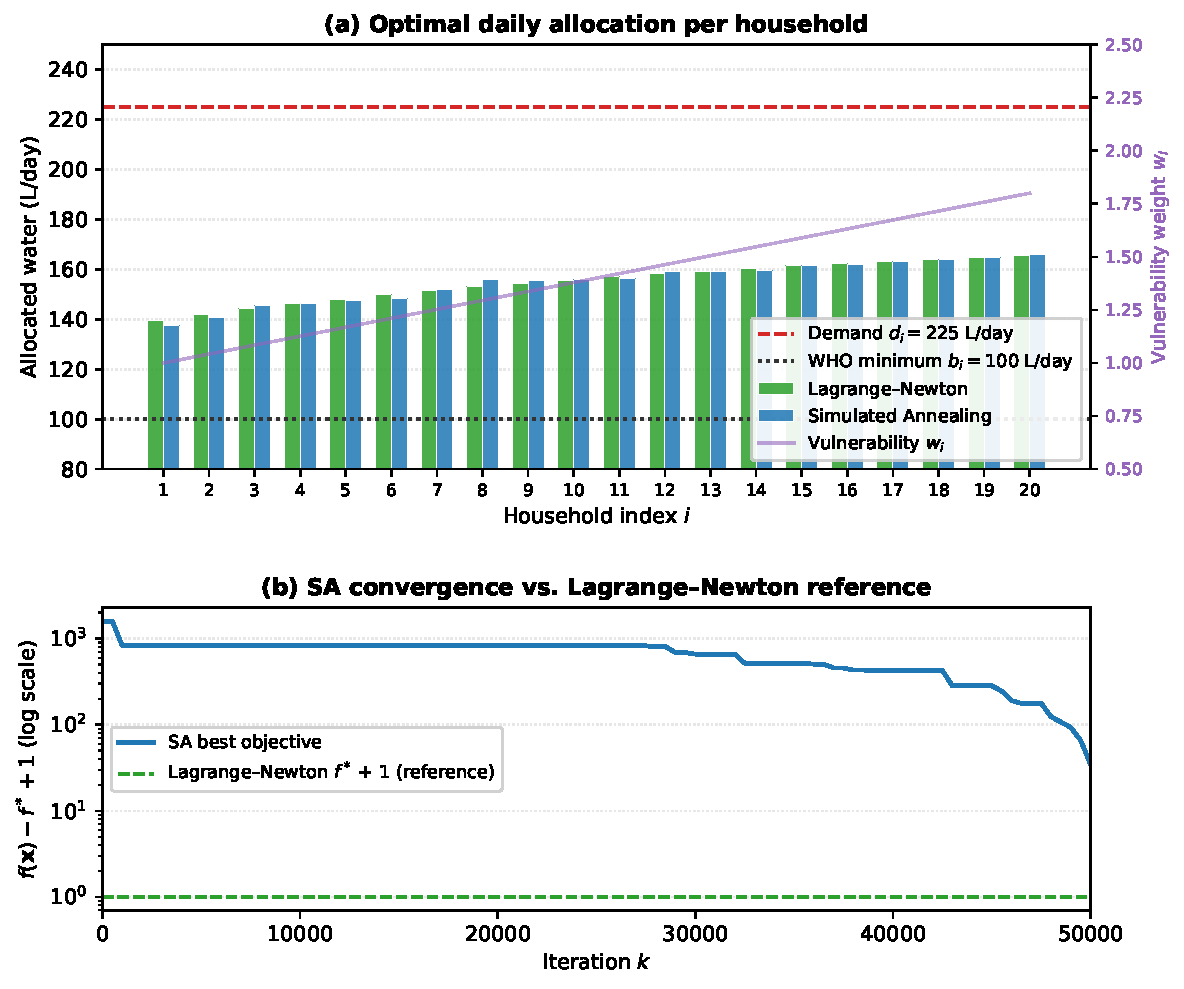
\includegraphics[width=0.65\linewidth]{Figures/allocation_and_convergence.pdf}
\caption{\textbf{Top:} Optimal daily allocation $x_i^{*}$ per
household for both methods; the dashed line marks the WHO
minimum $b = 100$~L/day, the dotted line the uniform demand
$d_i = 225$~L/day. \textbf{Bottom:} Convergence of the SA
objective compared to the Lagrange--Newton reference $f^{*}$
(log scale). Gap closes to $\approx 30\,\text{L}^2/\text{day}^2$ after $\sim\!15{,}000$ iterations.}
\label{fig:main}
\end{figure}

Both methods converge to essentially the same allocation
(Fig.~\ref{fig:main}, top). Because $S < \sum_i a_i d_i$ but
$S > \sum_i a_i b_i$, neither box bound is active in the base
scenario: every household sits strictly inside its box and
receives the interior water-filling
solution~\eqref{eq:waterfilling}, $x_i^{*} = d_i - \lambda^{*}
a_i / (2 w_i)$ with $\lambda^{*}\approx -170.81$ fixed
by~\eqref{eq:supply}. Higher-$a_i$ households are cut back more;
higher-$w_i$ households stay closer to their demand. Total
delivered water at the tap is $\sum_i x_i^{*} \approx
3{,}101$~\si{L/day}, which is less than $S = 3{,}500$: the
difference ($\approx 400$~\si{L/day}) is absorbed by pipe losses.
Key numbers are summarised in Table~\ref{tab:results}.

\begin{table}[H]
\centering
\small
\caption{Method comparison on the base scenario ($S=3500$).}
\label{tab:results}
\begin{tabular}{@{}lrr@{}}
\toprule
Metric & Lagrange--Newton & Simulated Annealing \\ \midrule
$f^{*}$ \quad(\si{L^2 / day^2})   & $133{,}446$      & $133{,}475$ \\
$\|\mathbf{x}^{*}_{\text{SA}} - \mathbf{x}^{*}_{\text{LN}}\|_{\infty}$ (\si{L/day}) & -- & $3.15$ \\
Iterations                        & $35$             & $50{,}000$ \\
Runtime (\si{\milli\second})      & $\sim 58$        & $\sim 835$ \\
Max.\ unmet demand (\si{L/day})   & $85.4$           & $87.5$ \\
Shadow price $|\lambda^*|$ (\si{L^2 \cdot day^{-3}}) & $170.81$ & -- \\
\bottomrule
\end{tabular}
\end{table}

The Lagrange multiplier $\lambda^* \approx -170.81$~\si{L^2\!\cdot day^{-3}}
is the shadow price of the supply constraint~\eqref{eq:supply}: one additional
litre per day of spring water reduces the total shortfall cost $f$ by
$|\lambda^*| = 170.81$~\si{L^2\!\cdot day^{-3}}, providing a direct
operational signal for infrastructure investment decisions.

The near-identical solutions are \emph{expected}, not a bug:
strict convexity guarantees a unique global minimum, so any
convergent method must reach it. This cross-validation is the
most informative outcome of the comparison.

\emph{Efficiency.}
Lagrange--Newton reaches the KKT point in $35$~iterations
and ${\sim}58$~\si{\milli\second}, orders of magnitude faster
than SA, whose budget of $50{,}000$ iterations is required for
the linear schedule to cool adequately.

\emph{Robustness.}
Varying the initial feasible guess $\mathbf{x}^{(0)}$ changes
SA's final $f$ by less than $0.04\,\%$ (max.\ gap $48$~L$^2$/day$^2$,
Table~\ref{tab:robustness}); Lagrange--Newton is
insensitive to $\mathbf{x}^{(0)}$ by convexity. Across supply
scenarios $S \in \{2500, 3500, 4500\}$~L/day both methods track
the analytic water-filling allocation smoothly
(Fig.~\ref{fig:scenarios}); at $S=2500$~\si{L/day} the lower box bound
is active for six households. The critical supply at which
the first bound activates is $S^* \approx 2784$~\si{L/day}, where
household~1 (lowest $a_i/w_i$ ratio) reaches $x_1^* = b_1$.

%--------------------------------------------------------------
\section{Discussion and Conclusion}
\label{sec:discussion}
%--------------------------------------------------------------

The fact that SA recovers the Lagrange--Newton optimum at
orders of magnitude higher computational cost illustrates a
textbook trade-off: on a smooth, strictly convex problem the
gradient-based method is strictly preferable~\citep{nocedal2006}.
SA's value in this project lies elsewhere --- it stress-tests
both the Lagrangian derivation (is the KKT solution we see
really the optimum?) and the feasibility-preserving move
operator~\eqref{eq:coupled}--\eqref{eq:deltamax}. Two natural
extensions push the model into regimes where SA becomes
competitive with, or superior to, Lagrange--Newton: \emph{discrete}
tap-placement decisions in the spirit of Laporte et al.~\cite{laporte2022}
turn the problem into a mixed-integer programme, and non-convex
pipe-loss models such as $\eta_i(x_i) = \alpha_i x_i / (1 +
\beta_i x_i)$ introduce local minima. In both cases KKT no
longer guarantees global optimality, and a metaheuristic
baseline provides a safety net that a local gradient method
cannot.

\emph{Limitations and conclusion.}
The model is static and deterministic: it ignores diurnal demand
peaks, storage dynamics, and stochastic spring yield, and the
weighted squared-deviation metric is one reasonable choice among
several (a max--min/Rawlsian alternative is left for future
work). With those caveats stated, we formulated household-level
fair water distribution in rural Nepal as a convex quadratic
programme with delivery-loss coupling and equity weights, solved
it with two methodologically distinct algorithms, and observed
the agreement that strict convexity predicts. Lagrange--Newton
is the production method; SA is the easily-extensible building
block for the non-convex extensions any real operational tool
would eventually require.


%==============================================================
% REFERENCES  (still part of main report)
%==============================================================
\bibliographystyle{unsrtnat}
\bibliography{references}

%==============================================================
% APPENDIX  -- separate numbering A-1, A-2, ...
%==============================================================
\restoregeometry
\appendix
\clearpage
\pagestyle{plain}
\pagenumbering{arabic}
\renewcommand{\thepage}{A-\arabic{page}}
\setcounter{page}{1}
%==============================================================
%  Appendix A -- Code & Supplementary Material
%  (does not count towards the 4-page limit, per the CO3 brief)
%==============================================================
\chapter{Supplementary Material}
\label{app:supp}

%--------------------------------------------------------------
\section{Lagrange--Newton implementation}
\label{app:code}
%--------------------------------------------------------------

Listing~\ref{lst:ln} reproduces the complete driver used to
produce the Lagrange--Newton results in
Section~\ref{sec:results}. The parameter vectors, objective,
gradient, constraint and solver call correspond one-to-one with
the formulation in Section~\ref{sec:formulation}. Both listings
are also available in the project repository:
\url{https://github.com/the-nerd-sloth/co3-semester-project.git}

\vspace{0.5cm}
{\captionsetup{justification=raggedright,singlelinecheck=false}
\lstinputlisting[
    style=pythonstyle,
    language=Python,
    caption={Lagrange--Newton baseline (\texttt{Code/lagrange\_newton.py}). Runs in $<1$~s on a standard laptop and reproduces the numbers quoted in Section~\ref{sec:results}.},
    label={lst:ln}
]{Code/lagrange_newton.py}}

%--------------------------------------------------------------
\section{Simulated Annealing implementation}
\label{app:sa}
%--------------------------------------------------------------

Listing~\ref{lst:sa} gives the self-contained SA driver.
The key design decisions are (i)~the feasibility-preserving
pairwise transfer move of equations~\eqref{eq:coupled}--\eqref{eq:deltamax},
which avoids \texttt{np.clip} after the perturbation step and
thereby keeps $\sum_i a_i x_i = S$ exact throughout; and
(ii)~the linear cooling schedule~\eqref{eq:cooling} with
$T_0 = 500$ and $k_{\max}=50{,}000$ as specified in CO3 Chapter~7.

\vspace{0.5cm}
{\captionsetup{justification=raggedright,singlelinecheck=false}

\lstinputlisting[
    style=pythonstyle,
    language=Python,
    caption={Simulated Annealing implementation (\texttt{Code/simulated\_annealing.py}).
    The constraint-preserving transfer move ensures strict feasibility at every step
    without any projection or rejection.},
    label={lst:sa}
]{Code/simulated_annealing.py}}

%--------------------------------------------------------------
% Supplementary tables and figures (no section headings --
% presented as self-contained floats with captions)
%--------------------------------------------------------------


\begin{table}[h]
\centering
\small
\caption{SA robustness across five independent random seeds
($S=3500$~L/day, $T_0=500$, $k_{\max}=50{,}000$, \texttt{step\_size}$=20$).
The gap $\delta f = f_{\text{SA}}^* - f_{\text{LN}}^*$ measures how far
each run is from the Lagrange--Newton reference $f_{\text{LN}}^* = 133{,}446$.
The maximum relative gap of $0.036\,\%$ confirms SA robustness to initialisation.}
\label{tab:robustness}
\begin{tabular}{@{}crrr@{}}
\toprule
Seed & $f_{\text{SA}}^*$ & $\delta f$ (L$^2$/day$^2$) & Relative gap (\%) \\ \midrule
 0  & 133\,466 & 20  & 0.015 \\
 1  & 133\,485 & 40  & 0.030 \\
 2  & 133\,494 & 48  & 0.036 \\
 3  & 133\,483 & 37  & 0.028 \\
42  & 133\,475 & 30  & 0.022 \\
\midrule
Mean & 133\,481 & 35 & 0.026 \\
\bottomrule
\end{tabular}
\end{table}

\begin{table}[h]
\centering
\small
\caption{Full 20-row allocation table for the base scenario ($S=3500$~L/day).
The vectors $\mathbf{a}$ and $\mathbf{w}$ are linearly spaced:
$a_i = 1.00 + 0.25\,(i-1)/(n-1)$ and $w_i = 1.00 + 0.80\,(i-1)/(n-1)$,
so that household~1 is the easiest to serve and least prioritised
while household~20 is the most pipe-lossy and most vulnerable.
Both methods produce the interior water-filling solution~\eqref{eq:waterfilling}
throughout; no box bound is active.}
\label{tab:full_alloc}
\begin{tabular}{@{}ccccrr@{}}
\toprule
$i$ & $a_i$ & $w_i$ & $d_i$ (L/day) & $x^*_{\text{LN}}$ (L/day) & $x^*_{\text{SA}}$ (L/day) \\ \midrule
 1 & 1.000 & 1.000 & 225 & 148.01 & 144.86 \\
 2 & 1.013 & 1.042 & 225 & 149.22 & 146.30 \\
 3 & 1.026 & 1.084 & 225 & 150.31 & 147.75 \\
 4 & 1.039 & 1.126 & 225 & 151.29 & 149.01 \\
 5 & 1.053 & 1.168 & 225 & 152.18 & 150.23 \\
 6 & 1.066 & 1.211 & 225 & 152.99 & 151.49 \\
 7 & 1.079 & 1.253 & 225 & 153.73 & 152.55 \\
 8 & 1.092 & 1.295 & 225 & 154.41 & 153.44 \\
 9 & 1.105 & 1.337 & 225 & 155.04 & 154.37 \\
10 & 1.118 & 1.379 & 225 & 155.62 & 155.30 \\
11 & 1.132 & 1.421 & 225 & 156.16 & 156.04 \\
12 & 1.145 & 1.463 & 225 & 156.67 & 156.84 \\
13 & 1.158 & 1.505 & 225 & 157.14 & 157.56 \\
14 & 1.171 & 1.547 & 225 & 157.58 & 158.21 \\
15 & 1.184 & 1.589 & 225 & 157.99 & 158.83 \\
16 & 1.197 & 1.632 & 225 & 158.38 & 159.53 \\
17 & 1.211 & 1.674 & 225 & 158.75 & 160.05 \\
18 & 1.224 & 1.716 & 225 & 159.10 & 160.67 \\
19 & 1.237 & 1.758 & 225 & 159.43 & 161.18 \\
20 & 1.250 & 1.800 & 225 & 159.74 & 161.77 \\
\bottomrule
\end{tabular}
\end{table}

\begin{figure}[h]
\centering
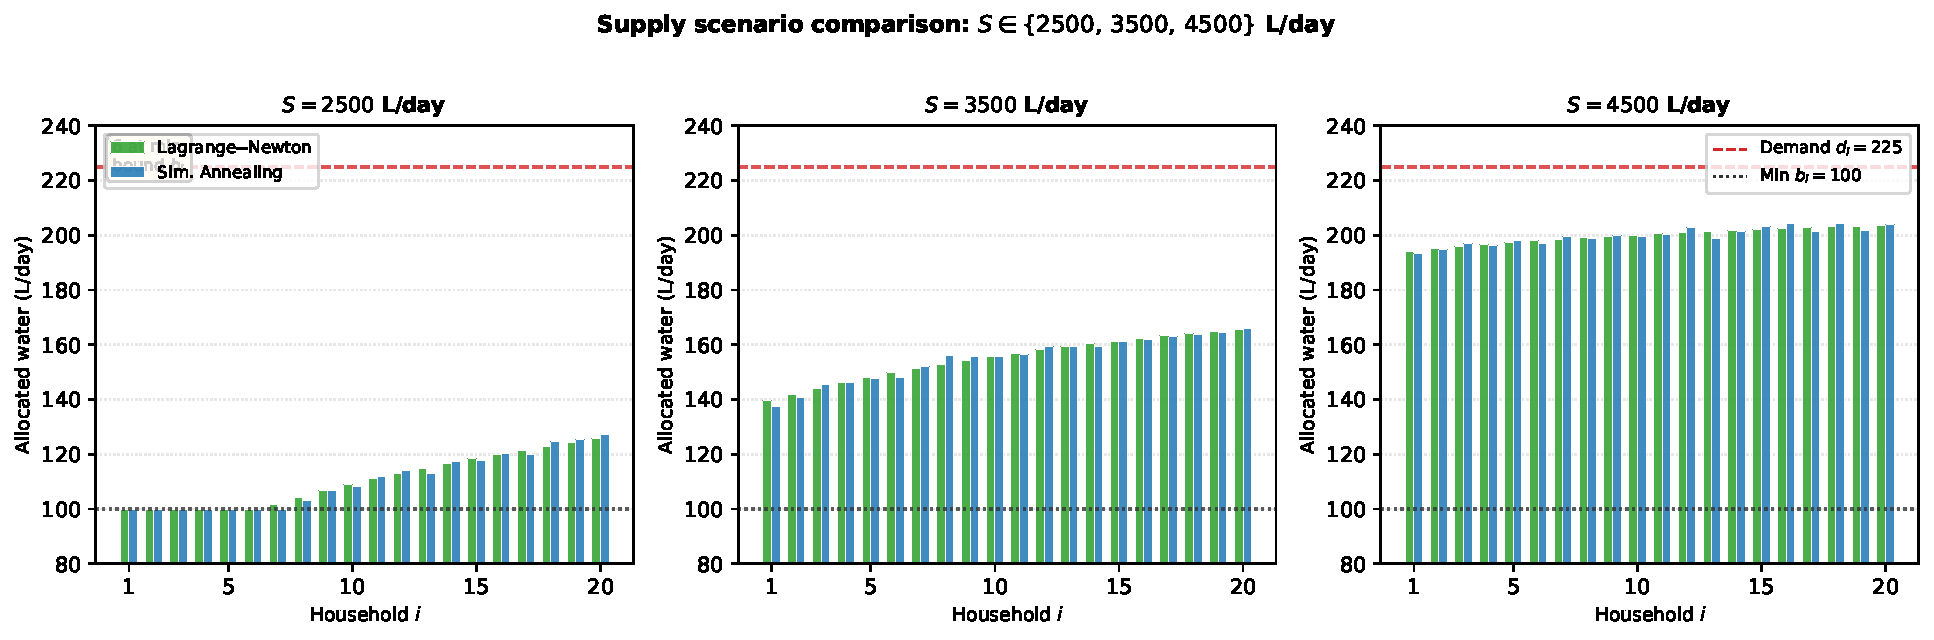
\includegraphics[width=\linewidth]{Figures/fig_scenarios.pdf}
\caption{Supply scenario comparison for $S \in \{2500,\,3500,\,4500\}$~L/day.
At $S=2500$~L/day (left panel) the lower box bound $b_i = 100$~L/day becomes
active for the six most pipe-lossy households ($a_i \geq 1.17$), confirming
the feasibility boundary analysis in Section~\ref{sec:formulation}.
At $S=3500$~L/day (centre) all households are interior and the water-filling
solution~\eqref{eq:waterfilling} applies throughout.
At $S=4500$~L/day (right) supply exceeds demand for the least pipe-lossy
households, but capping at $d_i=225$~L/day prevents over-delivery.
Both methods track each other closely across all three scenarios.}
\label{fig:scenarios}
\end{figure}

\begin{figure}[h]
\centering
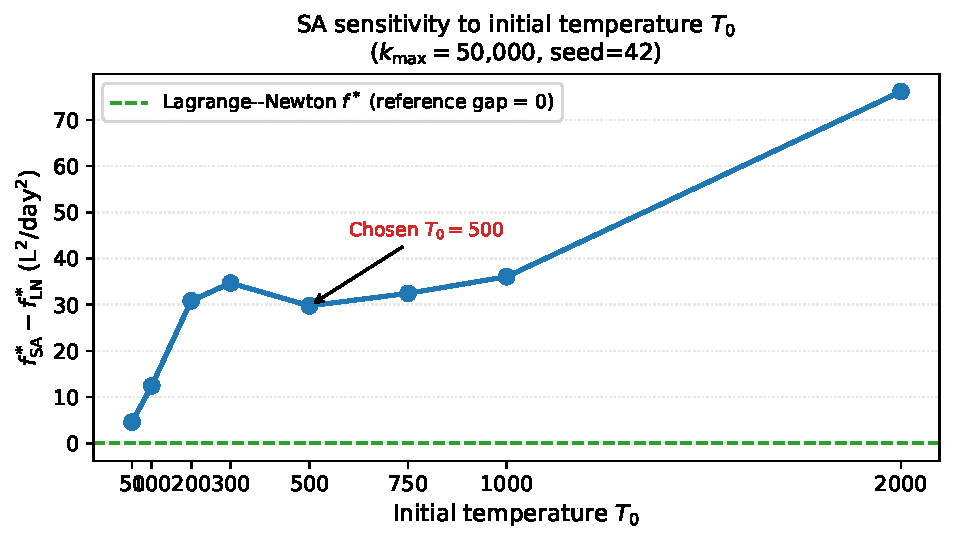
\includegraphics[width=0.72\linewidth]{Figures/fig_T0_sensitivity.pdf}
\caption{SA final objective gap $f_{\text{SA}}^* - f_{\text{LN}}^*$ as a
function of initial temperature $T_0$ ($k_{\max}=50{,}000$, \texttt{seed=42}).
The gap remains below $40$~L$^2$/day$^2$ across the full range tested,
confirming low sensitivity to $T_0$.  The chosen value $T_0=500$ (arrow)
balances early exploration with adequate final exploitation; very low $T_0$
($\leq 100$) reduces exploration and marginally increases the gap.}
\label{fig:T0}
\end{figure}


\end{document}
